\documentclass[conference]{IEEEtran}
\IEEEoverridecommandlockouts
% The preceding line is only needed to identify funding in the first footnote. If that is unneeded, please comment it out.
\usepackage{url}
\usepackage{cite}
\usepackage{amsmath,amssymb,amsfonts}
\usepackage{algorithmic}
\usepackage{graphicx}
\usepackage{textcomp}
\usepackage[ruled,linesnumbered]{algorithm2e}
\usepackage{xcolor}
\def\BibTeX{{\rm B\kern-.05em{\sc i\kern-.025em b}\kern-.08em
    T\kern-.1667em\lower.7ex\hbox{E}\kern-.125emX}}
\begin{document}
\title{
  What should I notice? Evaluating memorability of events for abductive inference.
}
\author{
  \IEEEauthorblockN{
  \IEEEauthorrefmark{1}\IEEEauthorrefmark{2} Étienne Houzé,
  \IEEEauthorrefmark{1} Jean-Louis Dessalles,
  \IEEEauthorrefmark{1} Ada Diaconescu,
  \IEEEauthorrefmark{2} David Menga
  }

  \IEEEauthorblockA{\IEEEauthorrefmark{1}
    Télécom Paris, IP Paris, \emph{Palaiseau}, France\\
  email: \{first\}.\{second\}@telecom-paris.fr}
  \IEEEauthorblockA{\IEEEauthorrefmark{2} EDF R\&{}D, \emph{Palaiseau}, France\\
  email: \{first\}.\{second\}@edf.fr}
}

\maketitle

\begin{abstract}
  When confronted to an unprecedented situation, humans typically show good
  performance in quickly identifying noticeable past events and proposing them
  as possible causal hypotheses. This kind of abductive inference is widely
  overlooked in modern AI approaches which rely on massive datasets to learn
  associative patterns. Our proposal is to formalize and compute a ``memorability''
  score over a memory of various recorded events from a cyber-physical system.
 This score can later be used either to select only relevant information to be
 remembered, or to propose causal hypotheses in unusual situations, on demand.
 As such, the approach aims at being complementary to more traditional
 learning-focused techniques. We provide theoretical ground for our approach by
 using and extending existing results and ideas from Algorithmic Information
 Theory and provide an implementation example, showing practical results in a
 smart-home scenario.
\end{abstract}

\begin{IEEEkeywords}
  Complexity, Algorithmic Information Theory, Simplicity, Abduction, Surprise
\end{IEEEkeywords}

\section{Introduction}

% As the number of connected devices and sensors grows, so does the amount of
% produced data. As a consequence, the ability to filter out a few events from past recordings
% as ``memorable'' becomes prime. While this task is often overlooked by many
% statistical approaches, which instead benefit from large quantity of
% information, it is part of the learning process for humans
% \cite{dehaene_how_2020}. Faced with new situations, humans are prone to infer
% previously seen unusual events as possible causes, and carry out further testing
% to assess the existence of a causal relation.


As a user has just turned on the TV in her all-equipped living-room, the
lights dim and the window blinds lower. Intrigued by this behavior, she
quickly infers that both light dimming and the blinds closing occurred as a
consequence of the TV being turned on. How did she come to this conclusion?
By performing \emph{abductive inference} \cite{magnani_abduction_2011}, which
is a key element of humans' ability to understand the world: from the
observed consequences, infer the possible causes.

In this example, there are mainly three possibilities to come to the
conclusion. If the user knows how the smart living-room system works, if she
knows the set of applied rules or parameters, she has access to a causal
knowledge she can use for the abduction. Otherwise, if she has no knowledge
about the system but the behavior occurs frequently, examining past
correlations will reveal that the television frequently causes the blinds to
close and the lights to dim. Else, if this is the first instance of the TV
being turned on in this living-room, there is no previous occurrence upon
which the user may rely to draw conclusions. However, she remains able to
infer the TV as a possible cause for the observed reaction: by noticing the
TV as a memorable recent event (since it is its first occurrence), she
proposes it as a possible cause for the questioned phenomenon. This example
shows how humans are able to use distinct methods to perform abductive tasks
and infer new knowledge. While abduction of the first two kinds can be
automated using knowledge bases and statistical approaches, this paper
proposes an approach to evaluate the memorability of events, allowing
machines to perform ``memorability-based'' abduction.




 % For instance, it is
% possible, for humans without any prior knowledge about
% physics or electrical engineering, to infer a memorable thunderstorm as a
% possible cause for a general black-out just by using the memorability of
% the former. While this kind of abductive inference (i.e. inference to the cause
% of an observation \cite{magnani_abduction_2011}) can yield many
% false-positives, it can be considered in situations where the lack of knowledge
% from previous occurrences penalizes other approaches.

% The difficulty of this approach to reasoning is, however, to quickly identify
% the relevant candidate hypotheses. In this regards, we may use a basic
% instinct: without prior knowledge, the most relevant hypothesis might simply be
% the most memorable recent event. However this definition is highly subjective,
% and does not seem to fit well into the canvas of computing and AI.

The difficulty of implementing this kind of abduction for machines comes from
several factors. First, events can be of different nature, and not directly
comparable. In fact, even for specific systems such as smart homes, events
range from device removal to a presence detection or an unusually high
temperature. How can one can then assess which ones are more memorable?
Furthermore, even for comparable events, different characteristics can be put
forward to argue for the most memorable: is a record-high temperature 47 days
ago more memorable than the small deviation recorded just 3 minutes ago? To
this day, no current system proposes to use all this information from various
event types from different devices to compute a unified metrics of
``memorability''.

% The difficulty of doing so comes from the wide variety of events, parameters and
% characteristics to take into account. How can one assess if a small recent
% perturbation is more important than a larger but older one? In addition, one
% needs a common metrics to evaluate the relative importance of data coming from
% various devices. In the case of a smart home, for instance, devices range from
% presence sensors to humidity and temperature sensors, power meters, etc. To this
% day, no current system proposes to analyze all events coming from such various
% devices and come to a unified metrics of ``memorability''.

% To tackle this challenge, we use as a starting point the observation that while
% all events, regardless of their characteristics or nature, can be uniquely
% described using a combination of qualifiers, the most memorable ones are likely
% to require less words to be described. Think, for instance, of ``last year's
% hottest day'' and ``the 182th day of 7 years ago''. By evaluating the lenght of
% each description, taking into account both the complexity of concept words (a
% time ranking, a temperature ranking), and the arguments used in both
% descriptions (the hottest, the 182th, 7), we can assign each event a complexity
% score. Memorable events, as they stand out, would then differ from their
% neighbors by being much simpler (or more complex).

To tackle this challenge, we rely on the following observation: while all
events, regardless of their characteristics or nature, can be uniquely
described using a combination of qualifiers, the most memorable ones are
likely to require less words to be described. Think, for instance, of
``last year's hottest day'' and ``the 182nd day from 7 years ago'': the
former seems simpler to describe. To quantify the notion, we can evaluate the complexity of each
description, taking into account both the complexity of concept words (a date
of occurrence, a temperature ranking), and the arguments (the hottest, the
182nd, 7). The resulting value defines the  \emph{description complexity}
of the events. As our intuition is that memorable events require simpler and less numerous qualifiers to be
unambiguously described than other unremarkable ones, they will stand out as simpler in terms of description complexity.

% A possible approach would be to rely on the naming complexity of events:
% memorable events are more likely to be shorter to be named than boring usual
% events. Think, for instance, of how ``last year's hottest day'' description
% appears much simpler than ``the 182th day of 7 years
% ago''\cite{robles_applications_2010}. Our idea is to rely on this metrics to
% estimate the description complexity of events. Then, by comparing the
% description complexity of a given event $e$ to the average complexity of similar
% events, we induce a measure of unexpectedness that can be used to assess the
% most memorable events.

\begin{figure}[ht]
  \centering
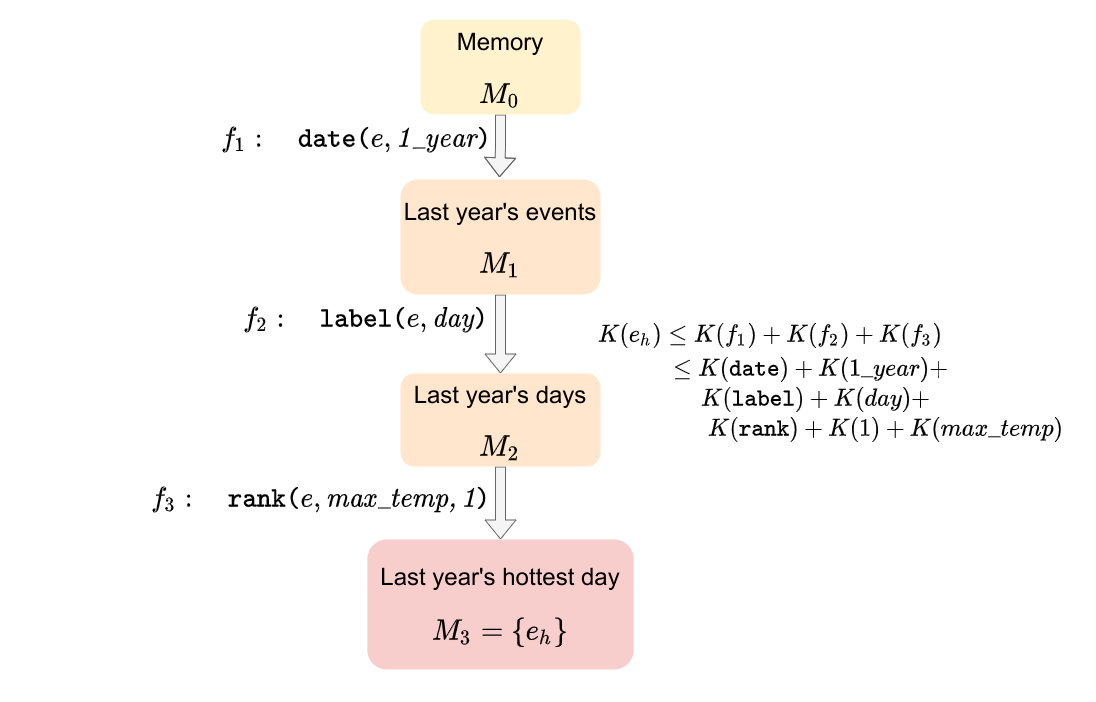
\includegraphics[width=\linewidth]{figures/filters}
\caption{Retrieving an event through successive predicative
filters. From the base memory (yellow), successive filters select events satisfying the associated predicate (grey arrows). For example,
   filter $f_1$ selects events from last year, i.e. which satisfy the
   predicate $\mathtt{date}(event, 1\_year)$. In this case, successively
   applying filters $f_1$, $f_2$ and $f_3$ yields a unique event $e_h$, last
   year's hottest day. The complexity of this event can then be upper bounded
   by the complexity of the three filters, since they give a unambiguous way
to describe the event in the memory.}
  \label{fig:filters}
\end{figure}

For machines to implement and compute description complexity, we need a formal canvas and computation methods which coincide with human intuition . To do so, we rely on Algorithmic Information Theory, which also appears to be consistent with the human perception of complexity\cite{li_introduction_2008,dessalles2011coincidences,delahaye_numerical_2012}. Our method is as follows: we
consider events as being unordered elements from a base \emph{memory}. To
reproduce the language features applicable to events, we use \emph
{predicates}, i.e. functions assigning a boolean value to an event and
eventual arguments. For instance, the predicate $\mathtt{date}
(\cdot, 1\_year)$ assigns \emph{true} to events that occurred last year. Selecting
all events, from the memory, that satisfy a given predicate corresponds to
a \emph{filter} operation, and yields another memory, a subset of the former.
This filtering operation can then be repeated, each iteration, selecting
fewer events, until a singleton memory is reached, meaning that the sequence
of predicates can \emph{retrieve} unambiguously the unique remaining event.
The description complexity of this event can thus be upper-bounded by the
number of bits required to describe the filters used in the retrieval
process. Figure \ref{fig:filters} illustrates this evaluation for the event
$e_h$: ``last year's hottest day''.



% To programmatically achieve this computation, we rely on principles from
% Algorithmic Information Theory, which provides formal definitions of complexity
% and simplicity of objects, which appear to be consistent with human perception
% \cite{li_introduction_2008, dessalles2011coincidences, delahaye_numerical_2012}.
%  Figure \ref{fig:filters} shows our solution applied to the example description
%  ``last year's hottest day''. We assume that
% a memory $\mathcal{M}$ is a unordered set of various distinct objects, upon
% which can be applied boolean predicates $\pi_{k}$ to describe them. These predicates thus
% provide filters $f_{\pi, k}$ that can be applied to the memory, selecting all events
% satisfying predicate $\pi_{k}$. By applying successive
% filters, we narrow down the size of the memory, until a single event remains.
% All the successive filters used to come to this singleton memory constitutes a
% \emph{retrieval path}, whose length, in bits, gives an upper bound of the
% description complexity of the retrieved event.

The rest of this paper is organized as follows: we first briefly introduce
some notions of Algorithmic Information Theory and its applications in
section~\ref{sec:theory}, then we explicit our methods to compute the
memorability of past events in cyber-physical systems~\ref
{sec:computing}. We illustrate this approach by providing an implementation
relying on a few predicates on events from a smart home simulation~
(section \ref{sec:example}). In section~\ref{sec:related} we briefly review
other related works using complexity theory or trying to explain smart homes
and how our work can be linked with them before exploring potential
extensions of our work in section \ref{sec:future}

\section{Theoretical Background}
\label{sec:theory}
Kolmogorov complexity formally quantifies the amount of information required
for the computation of a finite binary string\footnote{While the definition still
holds for some infinite binary strings (think of the representation of the
decimals of $\pi$), we restrict ourselves to finite strings in this paper.} (or
any object represented by a finite binary
string)\cite{kolmogorov_three_1965,li_introduction_2008}. For such a binary
string $s$, its complexity $K(s)$, is the bit length of the shortest program $p$
which, if given as input to a universal Turing Machine $U$, outputs $s$.
\begin{equation}
  \label{eq:kolmo_def}
  K_{U}(s) = \min_{p}\left\{l(p)|U(p)=s\right\}
\end{equation}

The first notable property of this definition is its universality: while the
choice of the Turing machine $U$ used for the computations appears in the
definition of eq. \ref{eq:kolmo_def}, all results stand, up to an additional
constant. Think, for instance, how any Turing-complete programming language can
be turned into any other language, using a compiler program. In fact, since any
Turing machine $U'$ can be emulated by $U$ from a
finite program $p_{U}$, we have the following inequality:
\begin{equation}
  \label{eq:inequality_univ}
  K_{U}(s) \le l(p_{u}) + K_{U}(s)
\end{equation}

From this first result, we can then define a universal complexity $K(s)$, which
no longer depends on the choice of a Turing machine $U$, such that, for any
machine $U$,
\begin{equation}
  \forall U\in\text{TM}, \forall s, |K(s) - K_{u}(s)| \le C_{U}
\end{equation}
where the additional constant $C_{U}$ does not depend on the object $s$.

It is important to note that the notion of Kolmogorov complexity is not related
to computation complexity, as there is no requirement on the execution time of
the programs, only their length in bits matters for the computation of
complexity. In fact, it can be shown that Kolmogorov complexity is not
computable\cite{li_introduction_2008}. The sketch of the proof is the
following: since the definition of complexity from Equation. \ref
{eq:kolmo_def} requires to find the shortest of all programs on a given Turing
machine outputting $s$, it requires to run all programs up to a given length
and compare their result to $s$. However, being able to do so means that we
would be able to tell whether these programs terminate. Since the termination
of programs is famously undecidable, by extension, the computation of
Kolmogorov complexity is impossible. One can however easily approximate it with
upper bounds, by exhibiting a program outputting $s$.

Interestingly, Kolmogorov's definition of complexity matches the intuitive
notion and perception of complexity from a human standpoint. For instance, the
complexity of short binary strings evaluated in \cite{delahaye_numerical_2012}
shows similar results to human perception of complex strings and patterns. More
recently, \cite{murena_solving_2020} used Kolmogorov complexity to solve
analogies and showed results close to human expectations.

This bridge between Algorithmic Information Theory and human perception of
complexity is extended to define the notion of simplicity and unexpectedness,
which are considered of uttermost importance in cognitive science\cite
{chater_simplicity_2003}.
\cite{dessalles2011coincidences} proposes a formal definition of the
 unexpectedness $U(e)$ of an event, as the difference between an a-priori
 expected causal complexity $C_{w}(e)$ and the actual observed complexity $C
 (e)$.
\begin{equation}
\label{eq:unexpected} U(e) = C_{w}(e) - C(e)
\end{equation}
This result comes from the understanding that, while Kolmogorov complexity is
computed with Turing machine, it can be used as an elegant proxy for modeling
information processing in the human brain, and thus helps design a notion of
simplicity or complexity of events.

The definition of Equation \ref{eq:unexpected} allows to model phenomenons
such as coincidences: imagine that you happen to run into someone in a park.
If this person has no particular link to you, the event will be quite
trivial: the complexity of describing this person will be equivalent to
distinguishing it from the global population, which will be roughly
equivalent as the complexity of describing that this person happens to be in
the same park as you. On the other hand, if you run into your best friend in
a park, as the complexity of describing your best friend is significantly
lower, the description complexity $C(e)$ drops while the causal complexity
remains $C_W (e)$ unchanged. Therefore the event becomes unexpected.

Using these insights from AIT, we define the memorability $M(e)$ of an event as the absolute difference between the description complexity $K_d(e)$ of an event and its expected description complexity $K_{exp}(e)$:
\begin{equation}
  \label{eq:memorability}
  M(e) = |K_{exp}(e) - K_d(e)|
\end{equation}
Contrary to the definition of unexpectedness from Equation \ref{eq:unexpected}, we use an absolute value: this is done to acknowledge events more complex than expected as memorable\footnote{In the original paper \cite{dessalles2011coincidences}, unusually complex events could be handled by considering complexity itself as a way to describe the event: see ``the Pisa Tower effect''\cite{dessalles_pisa_nodate}}. In the next section, we formally define the description complexity $K_d$ and the expected complexity $K_{exp}$ of events and detail how we can compute approximations of these quantities.

\section{Computing the memorability of events}
\label{sec:computing}
\subsection{Retrieving an event}

Computing the memorability of events begins with the introduction of formal definitions of events, how they are stored, how we can describe them and how these descriptions can be used to retrieve them.

We define \emph{events} as data points augmented with a \emph{label} indicating their nature (temperature event, failure event, addition/removal of a device) and a timestamp of occurrence. Formally:
\begin{equation}
  \label{eq:event}
  e = (l, t,\mathcal{D})
\end{equation}
where $l$ is the label, $t$ the timestamp and $\mathcal{D}$ a multi-dimensional data point representing the various characteristics of $e$: its duration, the maximum temperature reached, the sensor name, its position, etc. Labels can also be considered as classes of events, of which each event is a particular instance.

To model how humans are able to describe events by using qualifiers, we use \emph{predicates}: function operating on events, eventually taking additional parameters, returning a boolean value: $\pi(e, a_1, a_2, \dots, a_n) \mapsto \{O,1\}$ is a predicate of arity $n$ operating on event $e$. In the rest of this paper, we will prefer the equivalent notation $\pi(e, k) \mapsto \{0,1\}$, where $k$ is a binary string encoding the sequence of arguments $a_1, \dots, a_n$. Using this notation, the predicate $\pi$ becomes a boolean function operating on $\mathbf{E} \times \{0,1\}^*$:
\begin{equation}
  \label{eq:predicate}
  \pi : \begin{cases}
    \mathcal{M}\times \{0,1\}^{*} &\mapsto \{0,1\} \\
    (e, k) &\mapsto \pi_{k}(e)
    \end{cases}
\end{equation}
An example of predicate is to take $\pi = \mathtt{year}$ and $k$ a string encoding the number $1$, thus
constructing the predicate $\mathtt{year(}e, 1\mathtt{)}$, which tells whether
the event $e$ occurred $1$ years ago.

As events occur, they are stored in a \emph{memory} $M_0$. As they are not directly comparable, the memory $M_0$ can be considered as having the structure of an unordered set. We denote by $\mathcal{M}$ the subsets of $M_0$. By extension, elements of $\mathcal{M}$, i.e. subsets of $M_0$, are also called \emph{memories}.

By applying a given predicate $\pi_k$ to all events contained in a memory $M \subseteq M_0$, and selecting only events satisfying $\pi_k$ yields another memory $M_1 \subseteq M \subseteq M_0$. We call this operation a \emph{filter}:
\begin{equation}
  \label{eq:filter}
f_{\pi, k}: \begin{cases}
  \mathcal{M} & \mapsto \mathcal{M}             \\
  M           & \mapsto \{e \in M | \pi_k(e) \}
\end{cases}
\end{equation}
For instance, using the same $\pi = \mathtt{year}$ and $k=1$ as above, we can
build the filter $f_{\pi, k} = \mathtt{last\_{}year}$, which selects all events
that occurred last year.

As the output of a filter applied to a memory $M$ is another memory
object $M' \subseteq M$, we can compose filter
functions. A sequence of such filters is called a \emph{retrieval path}
\begin{equation}
\label{eq:ret_def}
p = (f_{\pi_{1}, k_{1}}, \dots, f_{\pi_{n}, k_{n}})
\end{equation}
and by definition
$p(M) = f_{\pi_{n}, k_{n}}(\dots(f_{\pi_{1}, k_{1}}(M)))$.
In case the result of the operation $p(M)$ contains a single element
$e$, we say that the path $p$ \emph{retrieves} the element $e$ from $M$, and write
$p(M) = e$. In the example shown in Figure \ref{fig:filters}, the three filters $f_1, f_2, f_3$ form a retrieval path retrieving the event ``last year's hottest day'' from the base memory $M_0$.

\subsection{Description complexity of events}

As presented in sec. \ref{sec:theory}, we are interested in computing an approximation of the description complexity of an event $e$. From the above definitions, if there is a path $p$ retrieving $e$ from the base memory $M_0$, i.e. $p(M_0) = e$, this path provides a possible unambiguous description for $e$. We therefore define the description complexity of $e$ as the minimum complexity of a path $p$ retrieving $e$ from the base memory $M_0$.

\begin{equation}
  \label{eq:k_desc}
  K_d(e) = \min_{p \in P_\infty} \{L(p) | p(M_0) = e\}
\end{equation}

where the bit-length $L(p)$ of a retrieval path is defined as the number of bits of a string encoding the path. If we limit ourselves to prefix-free strings encoding predicates and arguments, the total bit length is given by:
\begin{align}
  \label{eq:bit_lenght_p}
  L(p) & = L((f_{\pi_1,k_1}, \dots, f_{\pi_n, k_n}))     \\
       & = L(\pi_1) + L(k_1) + \dots + L(\pi_n) + L(k_n)
\end{align}


By considering only a finite number of possible predicates $\pi$ and arguments $k$, and a maximum path length, we can construct a finite set $P$ of possible retrieval paths. By limiting the search over this set, we can upper bound the description complexity, and use this upper bound as an approximation:

\begin{equation}
\label{eq:approx_k_desc}
K_d(e) \leq \min_{p \in P \land p(M_0) = e} L(p) = \min_{p \in P \land p(M_0)=e} \sum_{f_{\pi, k} \in p} L(\pi) + L(k)
\end{equation}

\begin{algorithm}
  $\mathtt{current_{explore}} \leftarrow [(\mathcal{M}, 0)]$ \;
  $\mathtt{future_{explore} \leftarrow} [\;]$ \;
  $\mathtt{pass} \leftarrow 0$ \;
  $\mathtt{K(e)} \leftarrow +\infty$ \;
  \While{$\mathtt{current_{explore}} \neq [\;]$ \textbf{and} $\mathtt{pass} < \mathtt{max\_pass}$}{
    \For{$(\mathtt{M_{prev}}, \mathtt{K_{prev}}) \in \mathtt{current_{explore}}$}{
      \For{$\mathtt{\pi \in \mathcal{P}}$}{
        \For{$\mathtt{k \in \{0,1\}^{*}}$}{
          $\mathtt{K_{current} \leftarrow l(\pi) + l(k) + K_{prev}}$ \;
          \If{$\mathtt{K_{current}} > \mathtt{max_{complex}}$}{
            \textbf{break} \;
          }
          $\mathtt{M'} \leftarrow f_{\pi,k}(\mathtt{M_{prev}})$ \;
          \eIf{$\mathtt{M'} = \mathtt{\{e\}}$}{
            $\mathtt{K(e) \leftarrow \min(K(e), K_{current})}$ \;
          }{
            $\mathtt{future_{explore}.append((M', K_{current}))}$\;
          }
        }
      }
    }
    $\mathtt{current_{explore}} \leftarrow \mathtt{future_{explore}}$ \;
    $\mathtt{future_{explore}} \leftarrow [\;]$ \;
    $\texttt{pass} \leftarrow \mathtt{pass} + 1$\;
  }
  \caption{Iterative computation of the approximate complexity}
  \label{alg:complex_iter}
\end{algorithm}

The approximation of description complexity from Equation \ref{eq:approx_k_desc} allows for
a direct implementation, which is shown in Algorithm \ref{alg:complex_iter}. This
algorithm operates iteratively: starting with the base memory $M_0$
(line 1), we apply all possible predicate concepts $\pi$ from a given finite set
$\Pi$ and programs $k$ (lines 6-7), up to a given length $\mathtt
{max\_len}$ bits, and apply them: $M' = f_{\pi, k}(M)$ (line 12). We then store
the pairs $(M', \mathtt{len(}\pi, k\mathtt{)})$ in an array $\mathtt{future_
{explore}}$. At the end of the iteration, the results of the filters become the
memories which will be explored during the next iteration(lines 21--23). Each
pass thus explore retrieval paths of increasing length. When a singleton memory
is reached, the complexity of its unique element is upper-bounded with the
length of the corresponding retrieval path (line 14).

\subsection{Computing Memorability}
As stated in Equation \ref{eq:memorability}, we define memorability $M(e)$ as the absolute difference between the description complexity of an event and its expected value. As we've just defined $K_d(e)$ and provided an approximation in Equation \ref{eq:approx_k_desc}, we now focus on defining the description expected complexity of an event, $K_{exp}(e)$.

As intended in the Equation \ref{eq:memorability}, this term evaluates the complexity the user, or the system, would expect the event $e$ to have without actually describing it, based on their previous knowledge. In our canvas, this prior knowledge consists of the base memory $M_0$. The expected complexity of the event $e$ can be computed with a simple first-order approximation, i.e. estimating the average complexity of ``similar events'' over the base memory $M_0$.

Still, difficulty remains in the definition of what
can be considered \emph{similar} events. Given that we deal with non comparable events, the only possibility to universally define the notion of similarity is to once again refer to \emph{predicates}. Thus, for a given event $e$, and a given predicate $\pi_k$, we define a $\pi_k$ neighborhood of $e$ as the set $N_{\pi, k}(e)$ of all other events satisfying $\pi_k$.

\begin{equation}
\label{eq:similar}
N_{\pi, k}(e) = \{e'\in M_0, \pi_k(e') \wedge e' \neq e\}
\end{equation}

Now, when considering, for all possible predicates $\pi_k$, the corresponding
neighborhoods $N_{\pi, k}(e)$, with the convention that $N_{\pi, k}(e) = \emptyset$
if $e$ does not satisfy $\pi_k$, we can compute an average expected complexity for $e$:

\begin{equation}
\label{eq:expected}
K_{exp}(e) = \frac{
\sum_{\pi, k} \sum_{e' \in N_{\pi, k}(e)} K_d(e')
                  }{
\sum_{\pi, k} |N_{\pi, k}(e)|
                  }
\end{equation}

This definition is consistent with the intuitive ideas that more similar events should weight more in the computation. Indeed, if $e'$
is \emph{very} similar to $e$, it will appear in many neighborhoods, since it
satisfies mostly the same predicates as $e$. Therefore, it will
be present in more terms in Equation \ref{eq:expected}, and will weight more in
the final result.

\subsection{From memorability to abduction}
% On peut étendre la définition utilisée pour la surprise en faisant intervenir
% les prédicats'' `sympathiques` par rapport à ce que l'on questionne.
The problem of the abductive inference is different from the basic computation
of the memorability score. Here, \emph{knowing} that we want to find a cause $c$
to an observed effect $e$, we try to find the most remarkable event in past
memory in that regard. While our ``memorability'' score aims to identify the
most remarkable events, it does not take into account the added knowledge about
the effect $e$ that is available for abductive inference.

This added knowledge can be integrated into the description complexity definition by using conditioned predicates. That is considering as given, and therefore ``free'' in terms of complexity, information contained in the cause effect $e$. For instance, when looking for a cause for
an anomaly in the living-room, other anomalies occurring in the same
living-room will be simpler, since the location ``living-room'' is already known
from knowing the consequence.

Formally, we now consider only predicates where knowledge of the effect event $e$  is appended to all programs $k$:
$\pi_{k::e}(c)$, where $::$ is the append operation. The set of paths obtained with such predicates is $P^\infty_e$. This append operation is free in terms of bit-length in the computation of complexity, since the effect event $e$ is an input of the problem. Therefore, we have $L'(\pi_{k::e}) = L(\pi_k) = L(\pi) + L(k)$. Which finally gives the definition for the conditional description complexity:

\begin{align}
  \label{eq:abd_k}
  K_d(c | e) & = \min_{p \in P^\infty_e} \{L'(p), \quad p(M_0)=c \}                                                \\
             & = \min_{p \in P^\infty_e} \left\{\sum_{f_{\pi, k::e} \in p} L(\pi) + L(k), \quad p(M_0) = c\right\}
\end{align}

This new conditional description complexity translates the additional information provided to the
system when answering a user's request. It can then be averaged over similar events to compute the expected conditional description complexity, $K_{exp}(c|e)$. From this, we come to the definition of the conditional memorability, which measures how memorable an event $c$ is, considering the knowledge of another event $e$:

\begin{equation}
\label{eq:cond_mem}
M(c|e) = |K_{exp}(c|e) - K_d(c|e)|
\end{equation}

Conditional memorability encapsulates the idea
presented as the motivation of this paper: when confronted to a surprising
situation, and with no other source of information, we can identify events that appear more memorable than others, with regards to the target effect event. As such, our conditional memorability score provides a ranking that can be used for abductive inference, proposing as best candidates the most memorable ones.

\section{Implementation Example}
\label{sec:example}
\subsection{Setup}
To test our approach, we set up an experimental smart home setup. This choice of
configuration is motivated by the challenges posed by smart homes for abductive
inference: i) as the number of connected devices increases, more events are
recorded, making the detection of memorable events more important; ii) smart
homes are prone to undergo atypical situations, highly dependent on the context,
for which pre-established relations might fail to find good abduction
candidates. Furthermore, the choice was also motivated by the ease of application: as
previous works exist on smart homes, it is possible to simulate their behavior
and quickly generate data to extract events from and test our methods.


% In order to provide an acceptable setup to our experiments, we used the scenario
% of smart homes. This kind of scenario is a prime example of situations where
% innovative methods of abduction can prove useful, for various reasons: i) as the
% number of sensors grows with the number of equipped devices in the house, not
% all recorded events are useful and should be remembered over long period of
% time; ii) atypical situations, which are the ones where abduction is most likely
% to be used (to explain situations to the user, or to solve a conflict), are also
% where the lack of past data makes knowledge acquisition hard.

To carry out the simulation, we built custom modules into the existing iCasa
smart home simulator\cite{lalanda_self-aware_2017}. This simulation platform
allows for simulating autonomic systems, handling internal communications,
injection of new components at runtime, deletion or change of existing
components. As such, we used a basic scenario consisting of a house of 4 rooms,
a single user, and an outdoor zone. All four rooms of the house are equipped
with a temperature controller system, monitoring and controlling heaters (fig.
\ref{fig:view}).

\begin{figure}[ht]
  \centering
  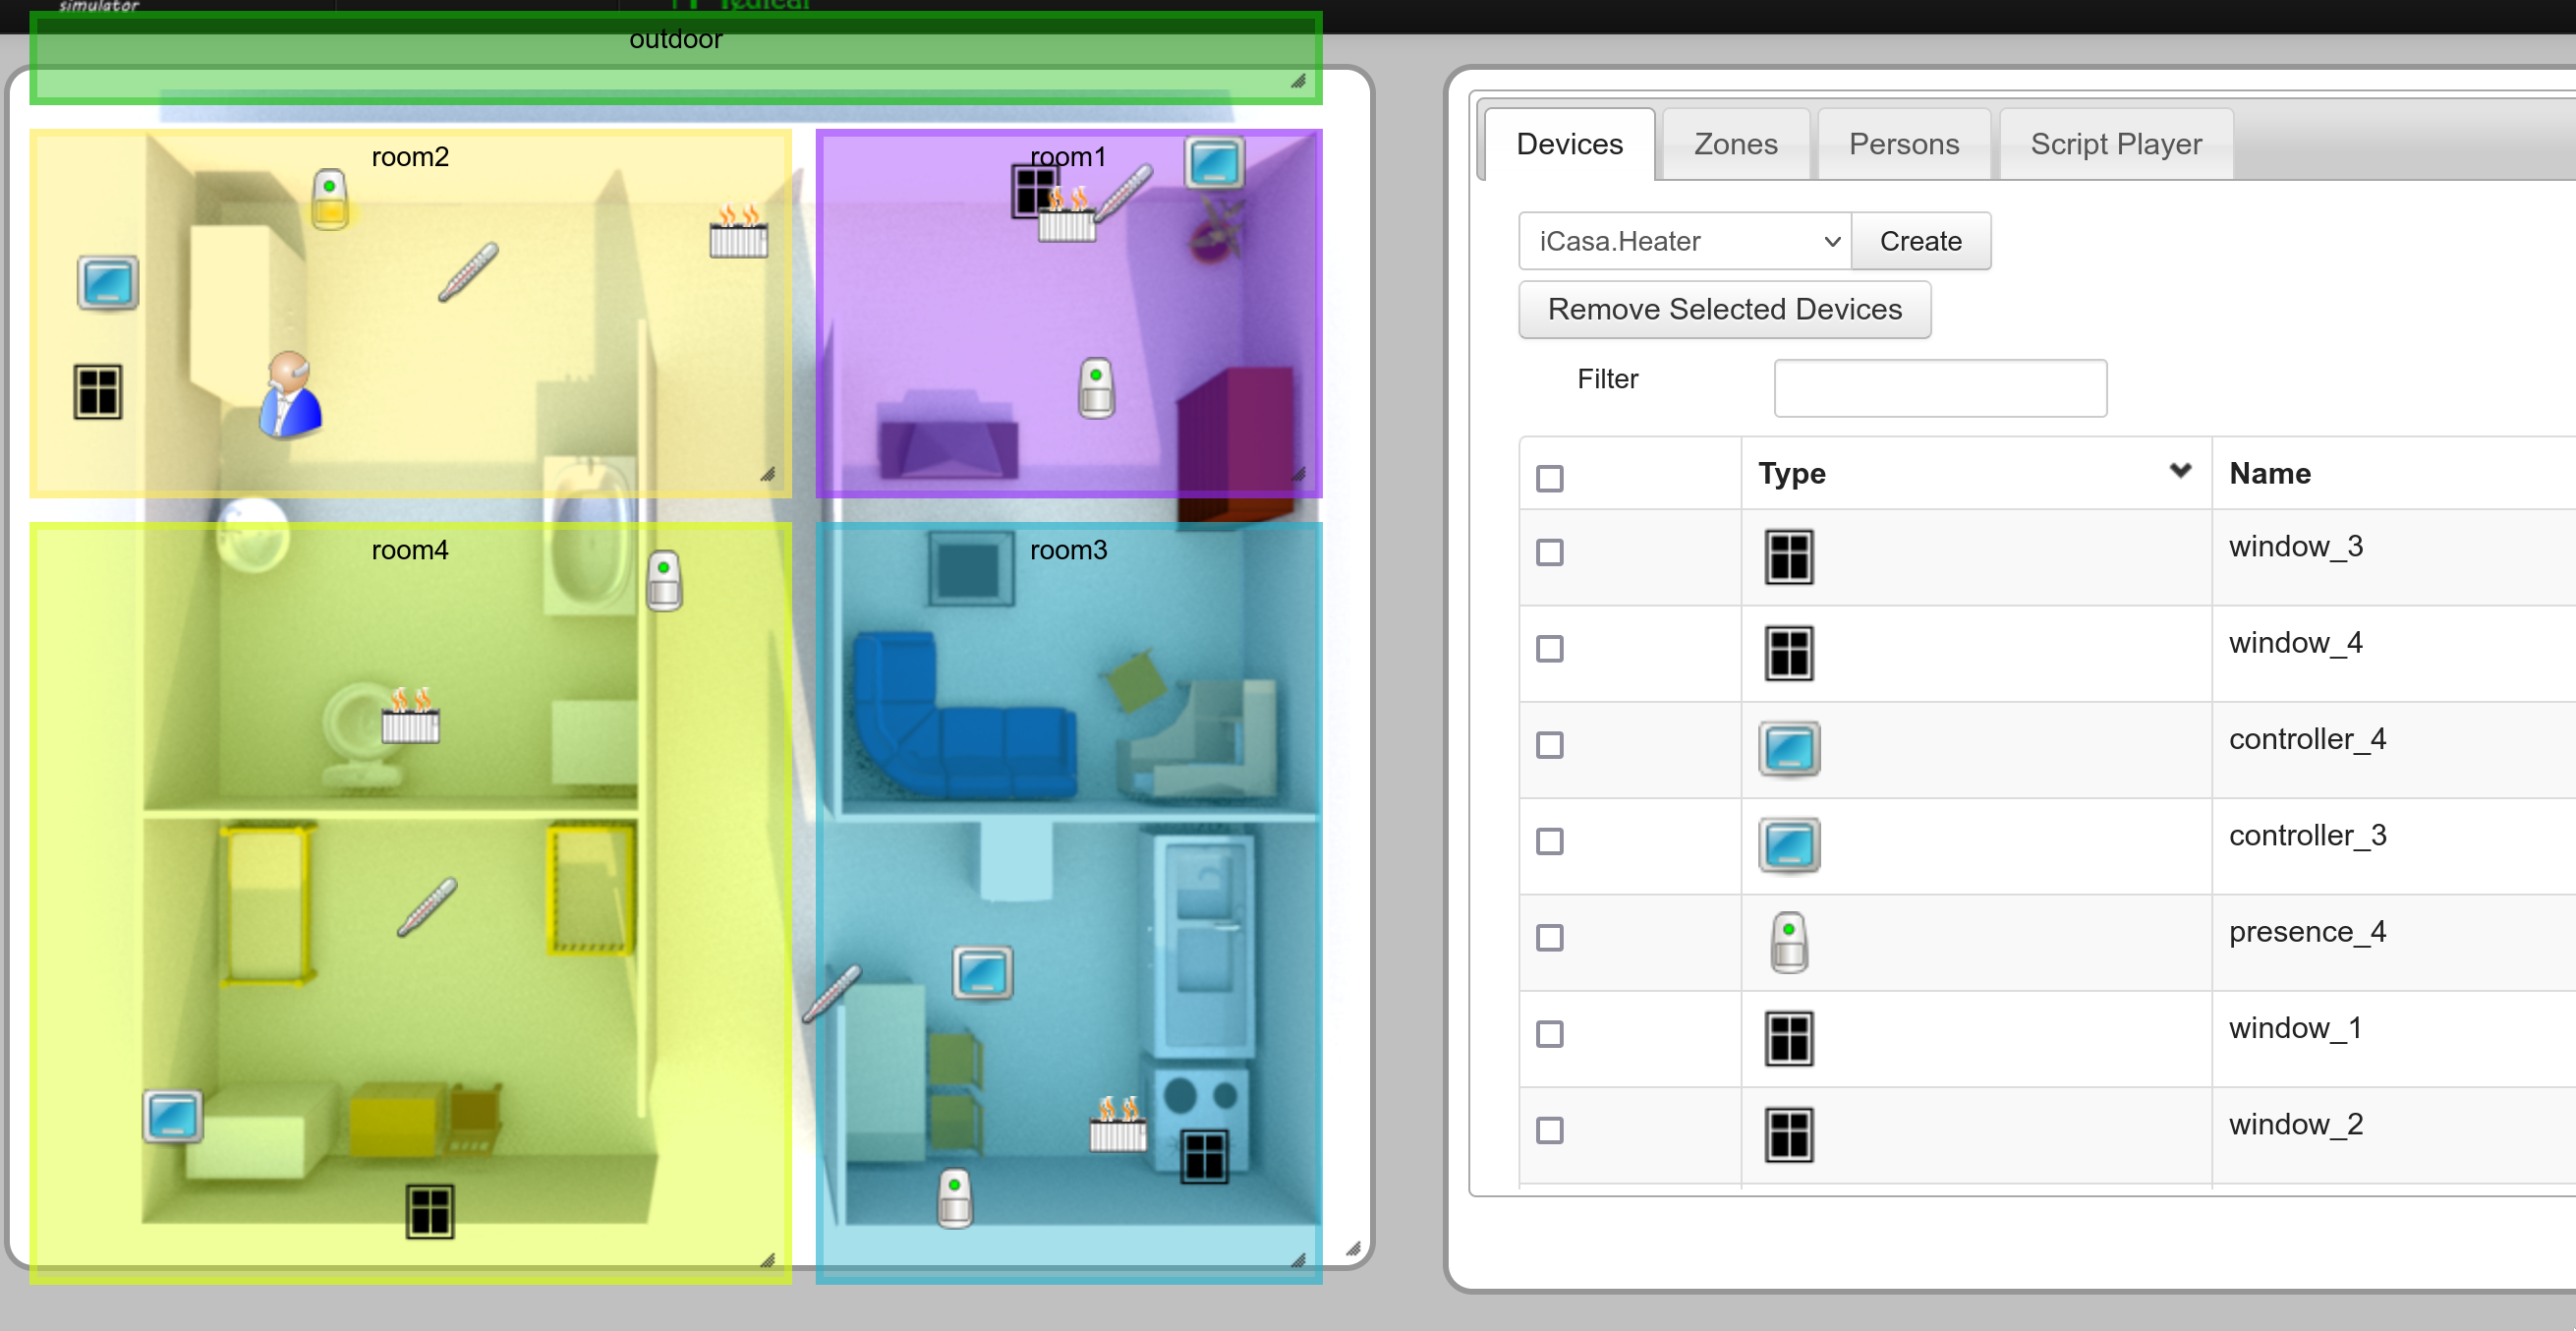
\includegraphics[width=\linewidth]{figures/simulator}
  \caption{View of the simulator's web interface provided by iCasa. The four
    rooms are visible, with their equipment and the user.}
  \label{fig:view}
\end{figure}

Using this basis, we implemented a scenario spanning over 420 days, and
comprising a daily cycle of outdoor weather (temperature and sunlight), as well
as user's movements. All these daily changes create non-noticeable events,
serving as a background noise for our experiments. To produce outstanding
events, we randomly generated around twenty events, spanning over the whole
duration of the simulation, of different kinds:

\begin{itemize}
    \item Unusual weather: the outdoor conditions are set to unusually high or
        low temperatures.
    \item Heater failures: heater can fail, making them turning off regardless
        of the command they receive.
    \item User's vacation: the user go out of the building for an extended
        period of time.
    \item Device removal/addition: a device is removed, or another one is added
        to the system.
\end{itemize}


\begin{figure}[ht]
  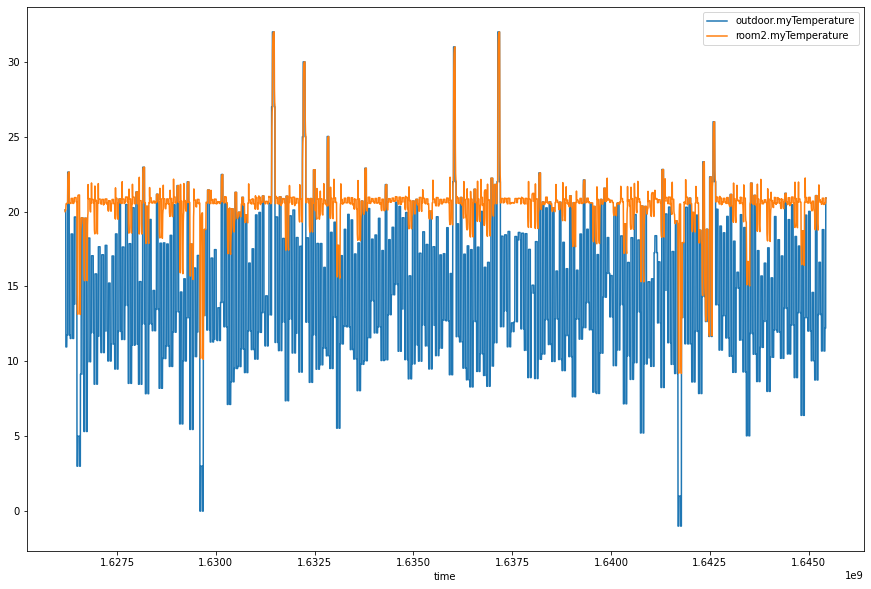
\includegraphics[width=\linewidth]{figures/ts_example}
  \caption{Time series data from the simulation: outdoor temperature (blue) and
controller temperature of a room (orange). On different occasion, the
    controlled temperature deviates from its setting (21°C). We will evaluate if
  our system finds these deviations as memorable, and if it can propose causal
  hypotheses.}
  \label{fig:ts_example}
\end{figure}

The values of all devices and zones variables was regularly monitored throughout
the simulation run, and the resulting data, which an excerpt is shown in figure
\ref{fig:ts_example} can later be used as a basis for our experiments.


\subsection{Implementing the complexity computation}

For the implementation of our method, we first needed to identify and
characterize events from the time series data generated by the iCasa simulation.
Since this is not the focus point of our present work (see sec.
\ref{sec:related}), we simply apply threshold and pre-computed conditions based
detection to create a set of events.

This set of events constitutes the basis of the initial memory $M_0$ used
for computations.
We then implemented a small number of predicate concepts:
\begin{itemize}
\item $\mathtt{label(e, k)}$: whether the event $e$ has the label ranked
        $k^{th}$ in the memory.
\item $\mathtt{rank(e, a_1, a_2)}$: whether the event $e$ has the rank $a_1$
along axis $a_2$.
\item $\mathtt{day(e, k)}$: whether the event $e$ occurred $k$ days ago.
\item $\mathtt{month(e, k)}$: whether the event $e$ occurred $k$ months
        ago.
\item $\mathtt{location(e, k)}$: whether the event $e$ occurred in zone
        $k$.
\end{itemize}

With a straightforward implementation of memory, predicates and filters, the
implementation of alg. \ref{alg:complex_iter} worked, but, as expected, took too
long to be usable in realistic scenarios with hundreds or thousands of events to
consider. In order to facilitate and speed up computations, we also implemented
the following improvements:
\begin{itemize}
  \item The memory object was augmented with various built-in rankings, allowing
  for faster operations during future filtering. For instance, since the memory
  object keeps a mapping from timestamps to events, which allows to quickly
  filter by date without having to loop over each stored element. This mapping,
  however, is not directly used to retrieve an event from the outside, as to
  preserve the theoretical model of memory as an unordered set presented in
  section \ref{sec:computing}.

  \item Each of these predicates holds the property that, in addition to
  \texttt{True} and \texttt{False}, they can return another value,
  \texttt{None}, which is theoretically treated as \texttt{False} but carries
  the additional information that this predicate concept will also be false for
  any other element of the memory for any subsequent program $k$. This allows to
  effectively break the innermost loop in alg. \ref{alg:complex_iter}.

  \item Some of the filters, for instance date or rank filters, were
  hard-written to select from the pre-computed mappings of the memory objects
  rather than testing a predicate over all memory elements.
\end{itemize}


\subsection{Results}

\subsubsection{Memorability}

The results of the description complexity evaluation, for the described setup,
are shown in fig. \ref{fig:computed_cplx}. The entire computation, over 4
iterations (meaning that retrieval paths contained at most 4 filters), took
around 30 seconds on a commercial laptop with an i7-8700u CPU.

A main sequence of ``usual'' events, which complexity is roughly a logarithm of
the elapsed time since their occurrence, is visible. This corresponds to events
for which the best retrieval path consists of a time description (e.g. ``2
months and 12 days ago''). On the other hand, some events stand out in terms of
complexity: some appear simpler, as they can be distinguished by using their
rank alongside an axis (``the hottest day'', ``the second longest user's
absence''), or the rare occurrence of their kind (``the only fault on the heater'').

\begin{figure}[ht]
  \centering
  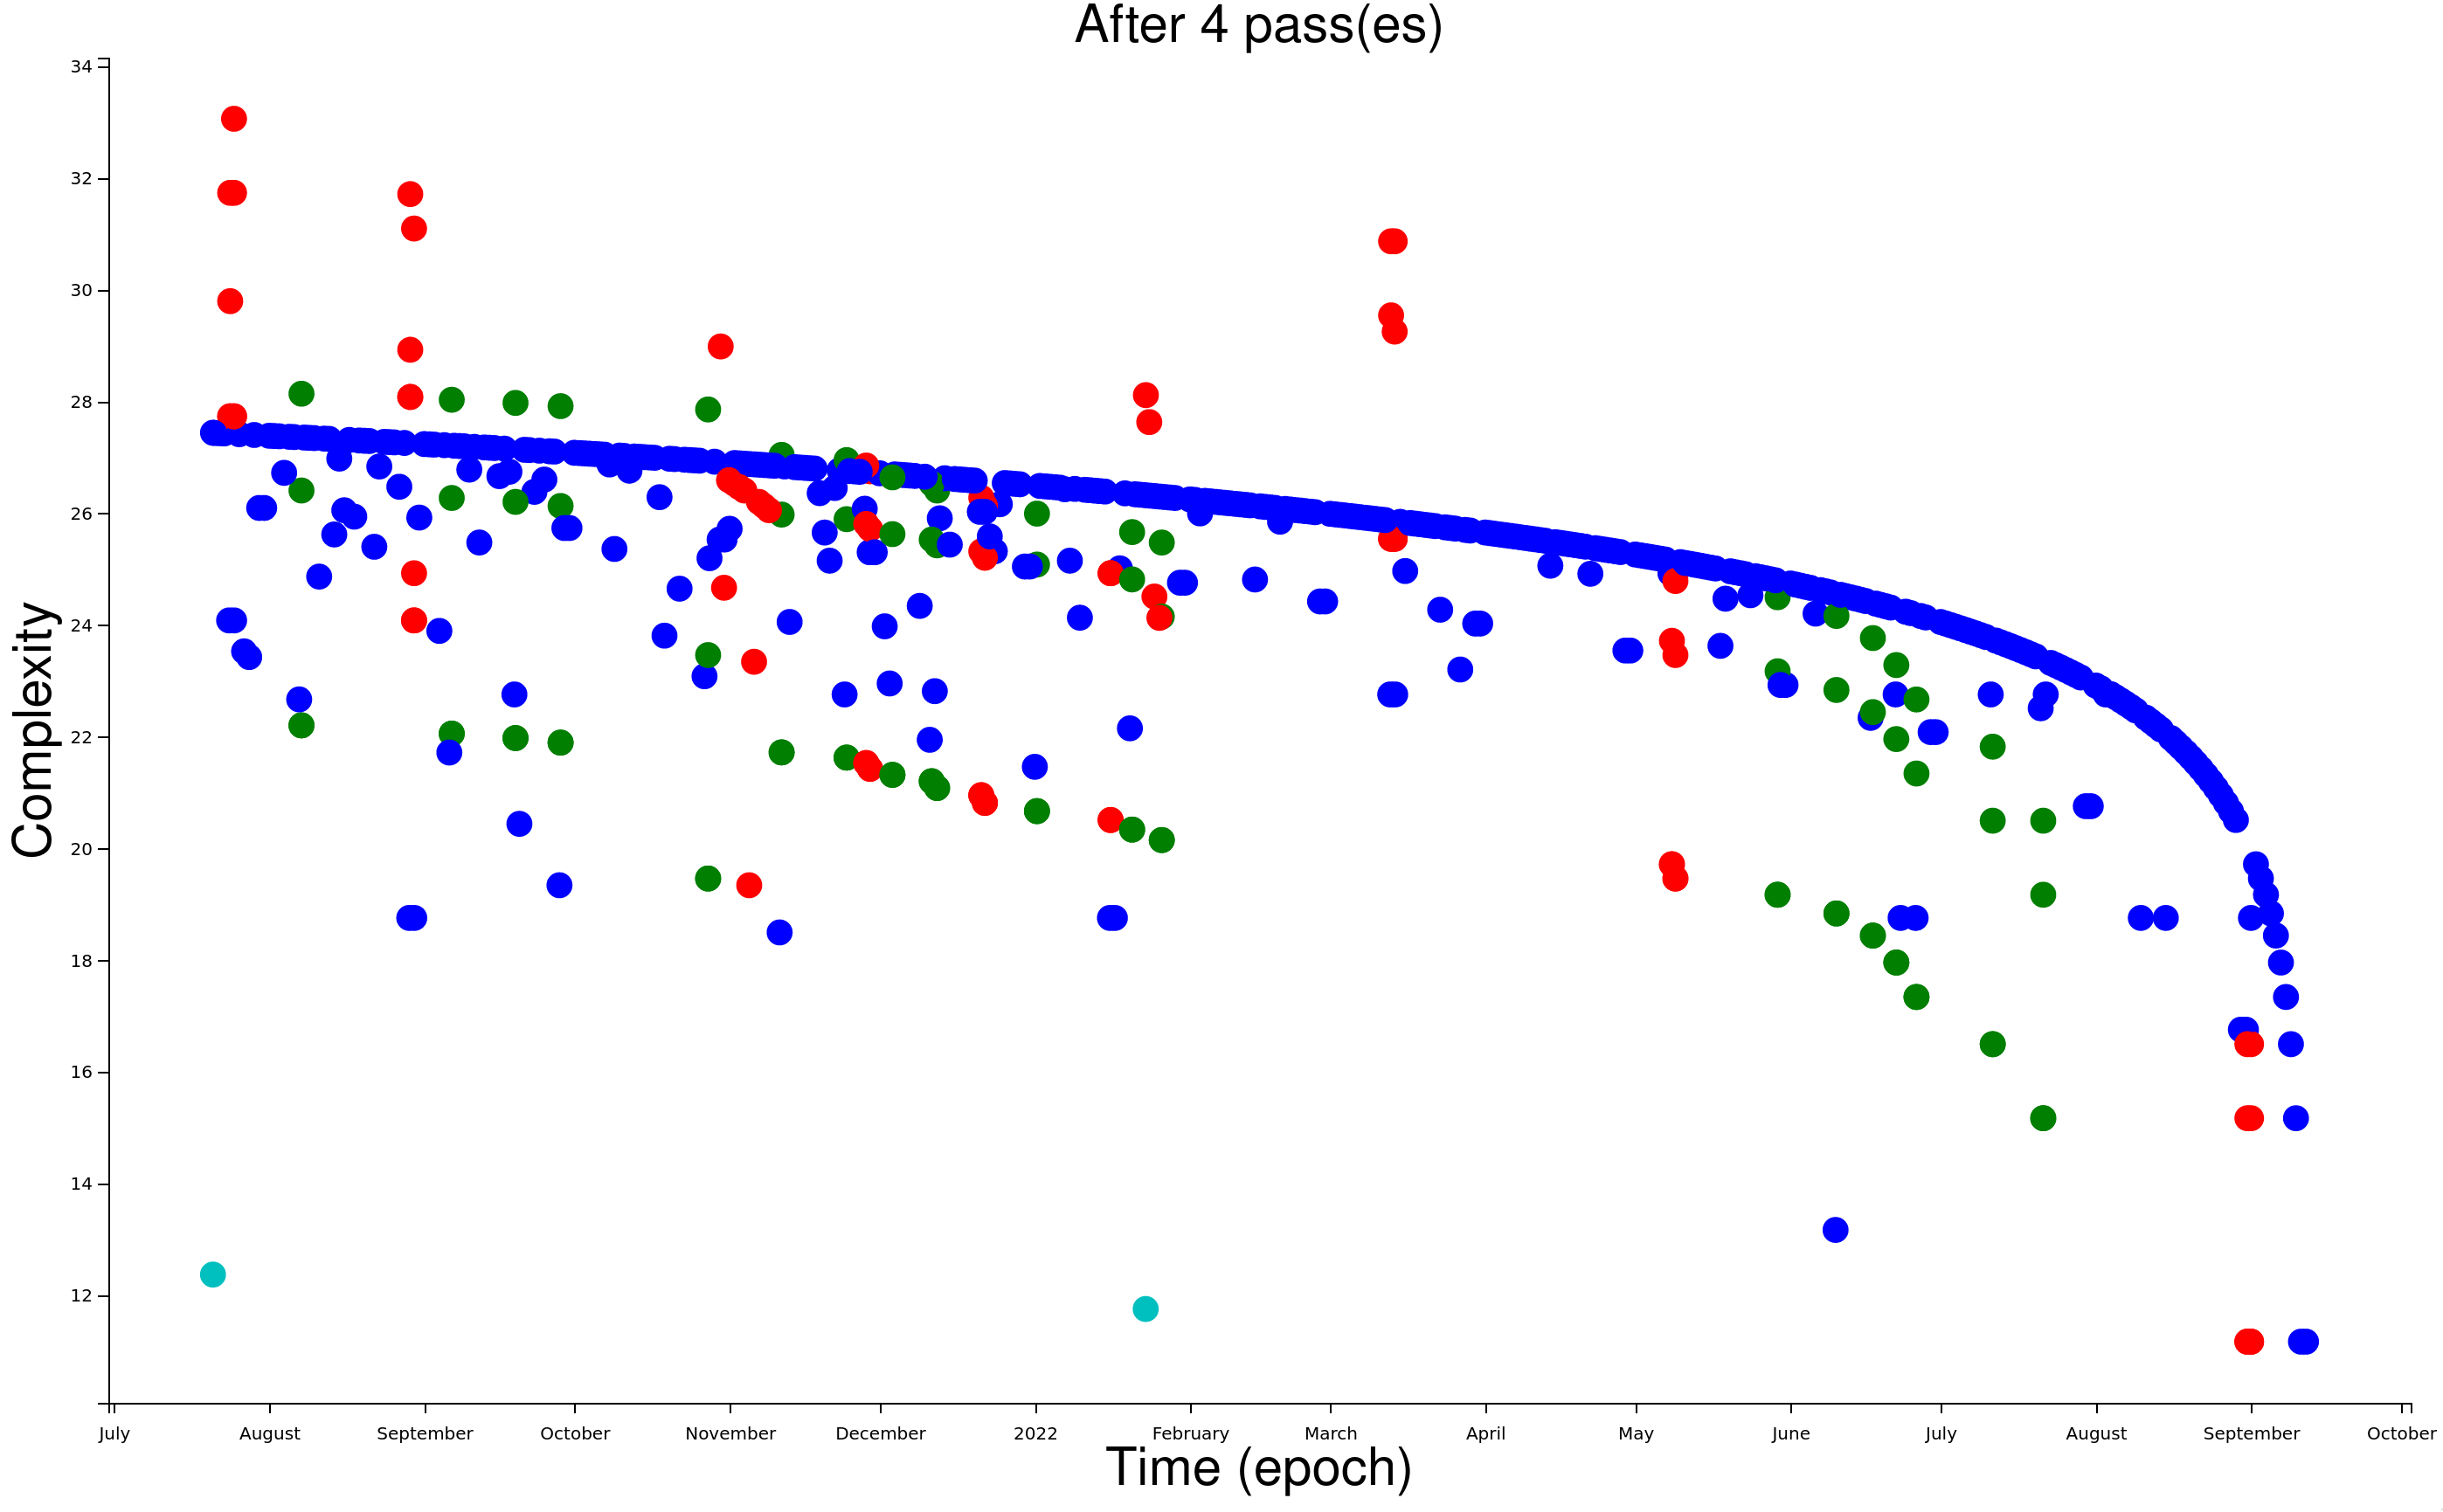
\includegraphics[width=\linewidth]{figures/complexities_computed}
  \caption{The computed complexities of events with at most retrieval paths of
    length at most 4. Events of type ``day'' (blue), ``hot'' (green), ``cold''
    (red), ``device removal''(cyan) are shown.}
  \label{fig:computed_cplx}
\end{figure}

Computing the ``memorability score'', which is shown in fig. \ref{fig:result1},
highlights these aforementioned events from the main ``usual'' sequence. Since
the computation of this measure treats unusually complex or simple events the
same way (from the absolute value operation in Equation \ref{eq:unexpected}), we
observe that some events are memorable due to their context only. For instance,
a temperature anomaly occurring simultaneously to many other anomalies is
notable, as it is costlier than expected to distinguish it from its neighbors.

\begin{figure}[ht]
  \centering
  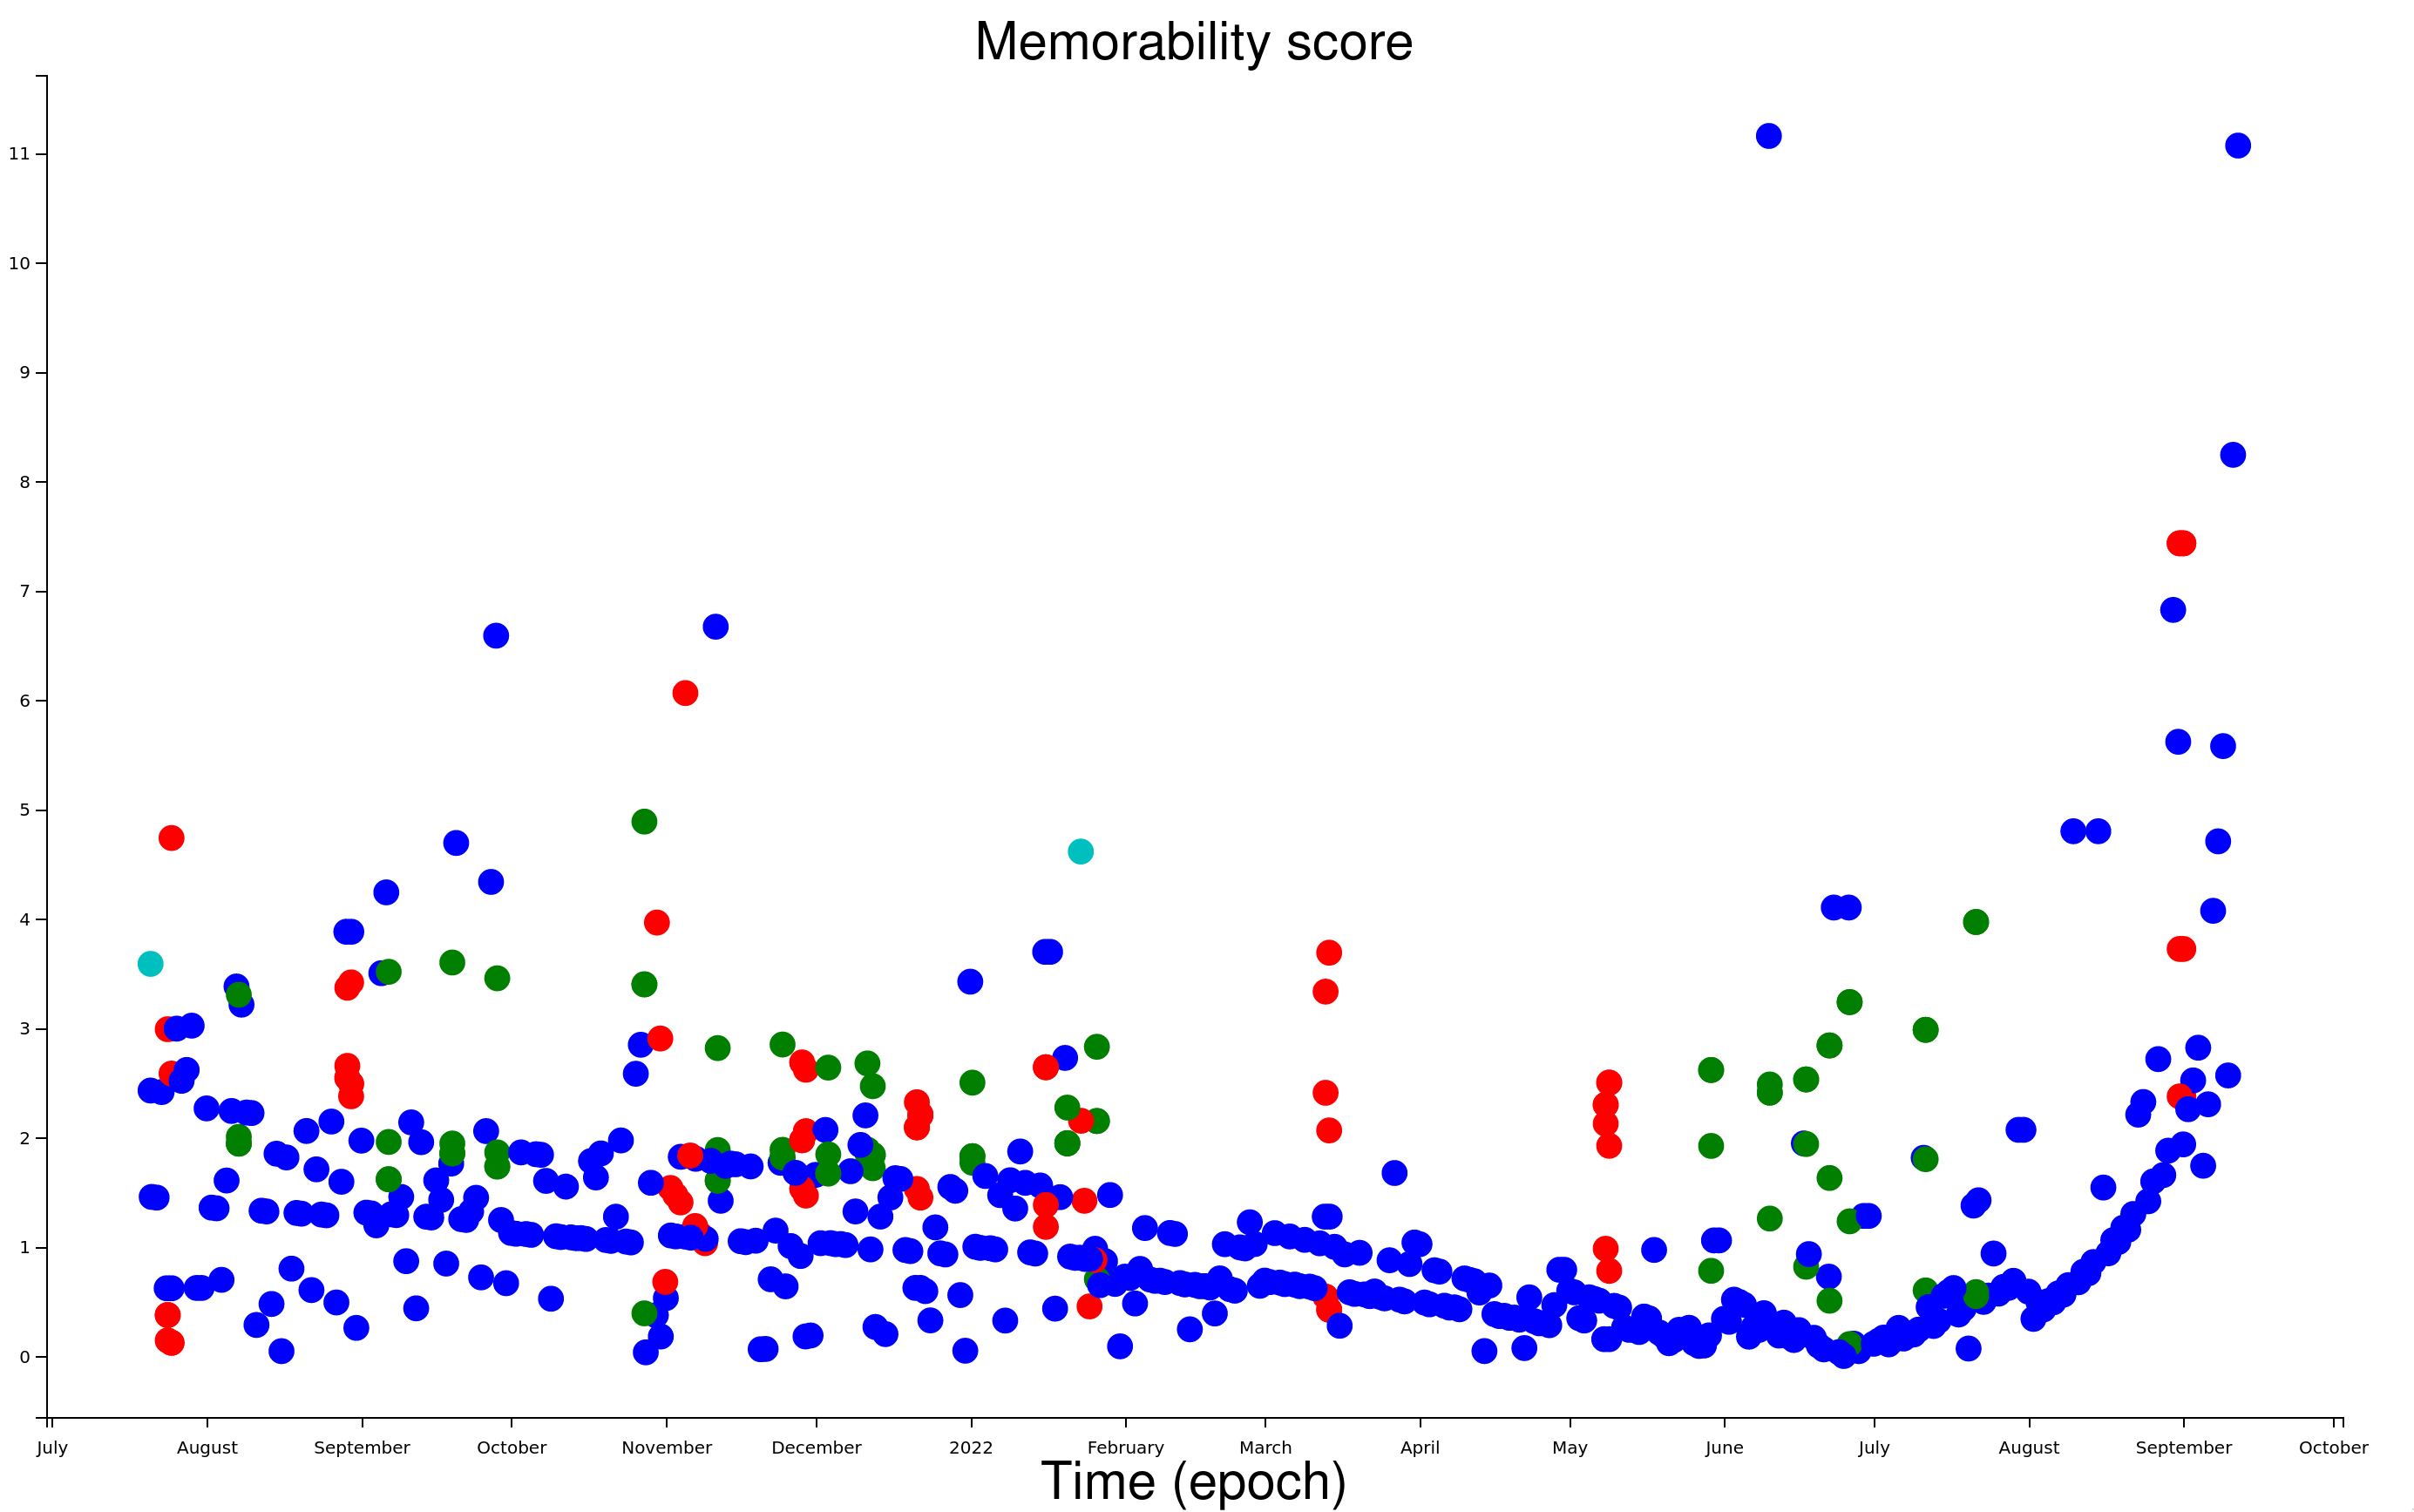
\includegraphics[width=\linewidth]{figures/complexities_surprises}
  \caption{Memorability score for events in the memory}
  \label{fig:result1}
\end{figure}

Given that we generated the data used for this experiment, it is possible to
flag all perturbation events from the usual daily events and evaluate how a
detection based on ``memorability'' score would succeed in distinguishing these
events. The result is presented as a ROC curve in fig. \ref{fig:roc}.

\begin{figure}[ht]
  \centering
  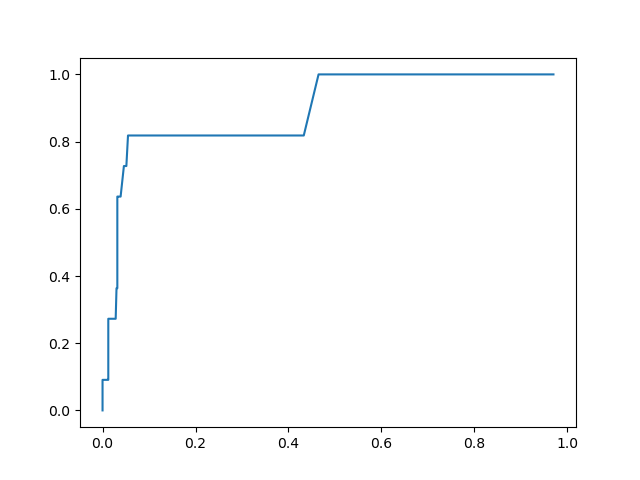
\includegraphics[width=\linewidth]{./figures/roc}
  \caption{Experimental ROC curve (True Positive Rate against False Positive
   Rate) for a classifier based on our memorability score. Measures consider 23
   manually flagged events as memorable (events added to the background noise
   as described in Section~\ref{sec:example}.)}
  \label{fig:roc}
\end{figure}
\subsubsection{Abduction}

As an illustration of the abductive inference possible by using the memorability
score, we used as a target consequence the temperature drop visible in the raw
time series data from our scenario (fig \ref{fig:ts_example}).

\textbf{TODO: the experiment still needs to be done: some additional data is required here (creating the scenario and finding causes.)}


\subsubsection{Discussion}
\label{ssub:discussion}

\section{Related Works}
\label{sec:related}
\textbf{TODO: this section is still WIP: I've added most references and short comments, but I still need to write the story linking them.}
Our work is intended to be integrated into larger-scale frameworks to monitor 
and detect events in complex environment such as smart homes. In these works, the
approach to smart homes is often regarded as self-organizing systems \cite{kramer_rigorous_2009,kounev_notion_2017}. As such, they present capacities of adaptation to new goals, 
new components, new environment. A commonly used approach is the principle of 
autonomic system, which minimizes user's intervention for management of the 
system \cite{kounev_notion_2017,kephart_vision_2003}.

We want to inscribe our work among other classical concurrent approaches to 
abduction. In situations where more data is available, we could for instance rely
on correlation or causal inference from known relations \cite{peters_elements_2017,fadiga_or_2021}.
Previous relations between inference and complexity have been studied. In fact, the 
case of inference was one of the motivations for R. Solomonoff to introduce his 
universal algorithmic probability \cite{solomonoff_formal_1964} as a tool to 
reach an idealized inference machine, creating the notion of complexity concomitantly 
to Kolmogorov. Subsequently, notions of complexity re-emerged in causal inference: 
\cite{janzing_causal_2010} found, when a causal link exists between two random variables,
considering the direct joint probability is simpler, in terms of Kolmogorov complexity, 
than the inverse direction.

More recently, \cite{marx_causal_2018} used Minimum Description Lenght to determine, given a joint probability distribution over $(X,Y)$, whether $X$ causes $Y$ or $Y$ causes $X$. Their method is based on tree models, and implying that a model respecting the causal relation will be simpler to describe.

\cite{tatti_finding_2008} PACK algorithm to cluster data using the simplest possible trees: maybe link this to isolation forests?

The topic of finding events from streams of time series data has already been explored in many ways. 
\cite{aggarwal_outlier_2017} provides good review of modern approaches and techniques
in the field. Some previous work can also be noted for having used AIT techniques to qualify and detect events in time series data. For instance, \cite{batista_complexity-invariant_2011,fadlallah_weighted-permutation_2013} propose weighted permutation entropy as a proxy for complexity measures in time series data, and use it to find relations between different time series. \cite{hu_discovering_2011} proposes a MDL approach to find the intrinsic dimensions of time series. All these approaches are interesting, and can be integrated into our canvas as tools to detect events using only complexity. As such, one could acheive a purely complexity-driven process for detecting and qualifying events.


Among various methods, the approach of ``Isolation forests''\cite{liu_isolation_2008,hariri_extended_2021} is closely related, by design, to ours. It evaluates the isolation of data points by constructing random binary tree classifiers. On average, outlier points will require less operations to be singled out. Using the average height of leaves in the tree as a metrics, this approach succeeds in identifying outlier points without having to define a ``typical'' point. This approach can be understood in terms of complexity: each node of binary tree classifier needs a fixed amount of information to be described (which variable and threshold are used). So nodes that place higher need less information to be described. As such, outliers need less information to be singled out. Compared to ours, this method is tailored for data-points living in the same metric space. By using predicates as a proxy for complexity computation, our methods is more general, as it is agnostic regarding the nature of events. However, the introdcution of predicates adds a subjectivity in the determination of memorable points, as we will discuss later.

While all these works advocate in favor of a strong link between complexity and the 
discovery of causes, not other works extends the notion up to the point we propose in this paper, using complexity only as a tool to express the intuitive notion of memorability, and using it for inference.

\section{Perspectives}
\label{sec:future}
The main purpose of the present paper is to show the possible connections
between existing definitions of simplicity from cognitive science, Algorithmic
Information Theory and a practical use case in cyber-physical systems. As such,
many further improvements can be done to pave the way towards a better
integration and performance for anomaly detection or abduction.

First, the main limitation of the current approach is the requirement of
predefined predicate concepts, from which the different filters are constructed.
As an extension, we suggest that in the future, we could explore online
generation of such predicate. A possibility would be to analyze discriminating
dimensions of incoming data and create predicate as to name these differences,
similar to the contrast operations proposed in \cite{dessalles_conceptual_2015,
  gardenfors2004conceptual}. For instance, the predicate concept $\mathtt{hot}$
can be discovered by discriminating a recent hot day along the
temperature axis and naming the difference with the prototypical day.

While the execution time is not part of the theoretical view of complexity, it
is of prime importance for practical applications, especially when one considers
implementation into real-time systems or embedded devices. While the computation
we propose appear to be heavy, and possibly heavier as the number of allowed
predicates grows, significant time savings can be achieve by trimming the base
memory of past events deemed the most ``non memorable''. For instance, one can
only retains the 100 most memorable events from the past. The difficulty with
this approach is that such operations should be done in a manner to not
interfere with the complexity computations for new elements: by forgetting some
past events, even uninteresting ones, one should make sure to keep track of what
made the interesting ones, interesting. Investigation of how to do so can pave
the way towards practical implementations and dynamic selection of interesting
events and help reducing the memory and computation cost of data-driven applications.


\section{Conclusion}


\bibliographystyle{IEEEtran}
\bibliography{biblio.bib}

\end{document}
